% ============================================================
%  REPORTE TÉCNICO: Clasificación de Texto con Redes Neuronales
%  Dataset: 20 Newsgroups (Dataset 3) | Framework: Keras / TensorFlow
%  Curso: Redes Neuronales - Universidad del Valle (2026-2)
%  Entrega 2: RNN sin memoria (SimpleRNN) y RNN con memoria (LSTM)
%
%  Compilar (en la carpeta proyecto2):   .\tectonic.exe RN2.tex
%  Las tablas y figuras se generan con analyze_e2.py (raíz del repositorio):
%  todo número de una tabla sale de un archivo de results/.
% ============================================================
\documentclass[12pt, a4paper]{article}

% ── Paquetes ────────────────────────────────────────────────
\usepackage[utf8]{inputenc}
\usepackage[T1]{fontenc}
% es-nodecimaldot: punto decimal en todo el documento (texto, fórmulas y tablas)
\usepackage[spanish, es-tabla, es-nodecimaldot]{babel}
\usepackage[margin=2.5cm]{geometry}
\usepackage{lmodern}
\usepackage{microtype}
\usepackage{amsmath, amssymb}
\usepackage{graphicx}
\usepackage{float}
\usepackage{booktabs}
\usepackage{array}
\usepackage{tabularx}
\usepackage{adjustbox}
\usepackage{xcolor}
\usepackage[colorlinks=true, linkcolor=blue, citecolor=blue, urlcolor=blue]{hyperref}
\usepackage{fancyhdr}
\pagestyle{fancy}
\fancyhf{}
\rhead{\small RNN sin memoria vs. RNN con memoria (Keras)}
\lhead{\small Reporte Técnico --- Entrega 2}
\cfoot{\thepage}
\setlength{\headheight}{15pt}
\setlength{\parskip}{6pt}
\setlength{\parindent}{0pt}

% Figuras y tablas generadas por el código
\graphicspath{{figuras/}}
\newcommand{\tabla}[1]{\input{tablas/#1.tex}}
% Tabla generada que se reduce solo si es más ancha que la página (ninguna tabla se sale del margen)
\newcommand{\tablaancha}[1]{\adjustbox{max width=\linewidth}{\tabla{#1}}}
% Nombre de una clase (grupo de noticias): monoespaciado y con cortes de línea permitidos en los puntos
\newcommand{\clase}[1]{\nolinkurl{#1}}

% ── Datos del documento ──────────────────────────────────────
\title{
    \textbf{Clasificación de 20 Newsgroups con Redes Recurrentes:} \\
    \large RNN sin memoria (SimpleRNN) frente a RNN con memoria (LSTM) en Keras \\[1em]
}
\author{
    John Ramos - 2370742\\
    Kevin Ramirez - 2324793 \\
    Dylan Morales - 2328330 \\\\
    \small Escuela de Ingeniería de Sistemas y Computación \\ Universidad del Valle\\
    \small \texttt{ramos.john@correounivalle.edu.co} \\
    \small \texttt{kevin.amaya@correounivalle.edu.co} \\
    \small \texttt{dylan.morales@correounivalle.edu.co}
}
\date{\today}

% ============================================================
\begin{document}

\maketitle
\thispagestyle{fancy}

% ── RESUMEN ─────────────────────────────────────────────────
\begin{abstract}
En la Entrega~1, un Perceptrón Multicapa (MLP) sobre vectores TF-IDF clasificó los mensajes de \textbf{20 Newsgroups} en sus 20 grupos sin tener en cuenta el orden de las palabras. En esta entrega se entrenan y evalúan, con los mismos datos, la misma partición y las mismas métricas, dos redes recurrentes que leen el texto palabra por palabra: una \textbf{RNN sin memoria} (SimpleRNN) y una \textbf{RNN con memoria} (LSTM). Las dos comparten el embedding, la capa de salida y las condiciones de entrenamiento; solo cambia la capa recurrente. La longitud de las secuencias, las unidades, el dropout y la tasa de aprendizaje se ajustaron uno a la vez con el F1 macro de validación, y el conjunto de prueba se usó una sola vez. Con la configuración final se probaron cuatro semillas de inicialización y, para cada red, se conservó la de mejor F1 macro de validación, que en ambos casos fue la 42. Con ella, en prueba, la LSTM obtuvo $50.08\%$ de exactitud y $49.32\%$ de F1 macro, el doble que la SimpleRNN ($25.21\%$ y $23.97\%$); el promedio de las cuatro semillas, más conservador, fue de $46.1 \pm 3.0\%$ frente a $20.7 \pm 2.4\%$ de F1 macro. Una prueba de memoria con distancia controlada muestra la causa: cuando a una frase con un tema claro le siguen 25 palabras sin relación, la LSTM todavía reconoce el tema en el $83\%$ de los casos y la SimpleRNN solo en el $21\%$. Ninguna de las dos superó al MLP de la Entrega~1, re-entrenado en el mismo entorno ($67.74\%$ de exactitud y $66.58\%$ de F1 macro): con 9\,616 documentos de entrenamiento y una mediana de 81 palabras por documento, este conjunto queda muy por debajo del tamaño a partir del cual la literatura recomienda modelos de secuencia, y para reconocer el tema de un mensaje importan más las palabras que contiene que su orden.

\textbf{Palabras clave:} 20 Newsgroups, redes neuronales recurrentes, SimpleRNN, LSTM, desvanecimiento del gradiente, clasificación de texto, Keras.
\end{abstract}

\tableofcontents
\newpage

% ============================================================
\section{Introducción}
% ============================================================

En la Entrega~1 se clasificaron los documentos de \textbf{20 Newsgroups} con un Perceptrón Multicapa (MLP) sobre vectores TF-IDF. Ese modelo alcanzó $68.03\%$ de exactitud y $66.90\%$ de F1 macro en el conjunto de prueba (configuración \textit{Tuned}), pero tiene una limitación de fondo que el propio reporte señaló: TF-IDF representa cada documento como una bolsa de palabras y descarta su orden. Las frases ``\textit{The doctor treated the patient}'' y ``\textit{The patient treated the doctor}'' producen exactamente el mismo vector.

Las redes neuronales recurrentes (RNN) leen el texto palabra por palabra y mantienen un estado que resume lo leído, por lo que sí dependen del orden. El enunciado de la Entrega~2 pide entrenar y evaluar dos modelos sobre el mismo conjunto de datos: una \textbf{RNN sin memoria} y una \textbf{RNN con memoria} (LSTM, GRU o Transformer). En este trabajo se usan:
\begin{itemize}
    \item una \textbf{SimpleRNN} (red de Elman~\cite{elman1990}) como RNN sin memoria: tiene un estado oculto que se reescribe en cada paso, sin celda de memoria ni compuertas;
    \item una \textbf{LSTM}~\cite{hochreiter1997} como RNN con memoria: agrega una celda de memoria controlada por compuertas, diseñada justamente para conservar información a lo largo de secuencias largas.
\end{itemize}

Para que la comparación sea justa, los dos modelos comparten todo excepto la capa recurrente, y se usan los mismos datos, la misma partición y las mismas métricas de la Entrega~1, de modo que también pueden compararse con el MLP. Cada decisión de diseño se acompaña de su justificación: el enunciado, la Entrega~1, la documentación o la literatura, una medición sobre los datos o el resultado en el conjunto de validación.

El reporte está organizado así: la Sección~\ref{sec:datos} describe los datos y cómo se convierten en secuencias; la Sección~\ref{sec:fundamentos} resume la teoría de las dos redes; las Secciones~\ref{sec:arquitectura} y~\ref{sec:entrenamiento} presentan las arquitecturas y las condiciones de entrenamiento; la Sección~\ref{sec:ajuste} describe el ajuste de parámetros; la Sección~\ref{sec:resultados} presenta y analiza los resultados; la Sección~\ref{sec:demo} describe la demostración y la Sección~\ref{sec:conclusiones} cierra con las conclusiones.

% ============================================================
\section{Conjunto de datos y preprocesamiento}\label{sec:datos}
% ============================================================

\subsection{Datos y partición}

Se usa la versión de 20 Newsgroups~\cite{lang1995newsweeder} que distribuye scikit-learn~\cite{pedregosa2011scikit}: 18\,846 mensajes de 20 grupos de noticias, separados por fecha en entrenamiento (11\,314) y prueba (7\,532). Como en la Entrega~1, se quitan encabezados, firmas y citas (\texttt{remove=("headers", "footers", "quotes")}), tal como recomienda la documentación de scikit-learn para que la evaluación sea realista~\cite{sklearn20ng}: esos metadatos delatan el grupo de origen. Del conjunto de entrenamiento se separa un $15\%$ estratificado para validación con la semilla 42 de la Entrega~1, lo que deja 9\,616 documentos para entrenar, 1\,698 para validar y 7\,532 para la prueba final. El conjunto de prueba solo se usa una vez, al final, con los modelos ya elegidos.

\subsection{Del texto a las secuencias}

El MLP recibía un vector TF-IDF por documento; las RNN necesitan la secuencia de palabras. Cada texto se convierte en una lista de enteros (uno por palabra) con la capa \texttt{TextVectorization} de Keras, ajustada solo con el conjunto de entrenamiento, y se recorta o rellena a una longitud fija $L$. La Tabla~\ref{tab:decisiones_datos} resume las decisiones de esta etapa y de dónde sale cada una.

\begin{table}[H]
\centering
\caption{Decisiones del preprocesamiento y su justificación.}
\label{tab:decisiones_datos}
\small
\begin{tabularx}{\linewidth}{>{\raggedright\arraybackslash}p{2.6cm} >{\raggedright\arraybackslash}p{4.2cm} X}
\toprule
\textbf{Decisión} & \textbf{Valor} & \textbf{Justificación} \\
\midrule
Tokenizador & \texttt{TextVectorization}: minúsculas y sin puntuación & Opción por defecto de Keras~\cite{kerasdocs}. \\
Vocabulario $V$ & 20\,000 palabras (incluye el relleno y la palabra desconocida \texttt{[UNK]}) & Es el tamaño del ejemplo oficial de Keras con este mismo conjunto de datos~\cite{kerasglove}; la EDA confirma la cobertura (Tabla~\ref{tab:eda_V}). \\
Longitud $L$ & Se prueban 100, 200 y 400 tokens & Rango tomado de la distribución de longitudes (Figura~\ref{fig:eda}); el valor final de cada modelo sale de validación (Sección~\ref{sec:ajuste}). \\
Relleno y truncamiento & Ceros a la derecha; si el texto es más largo se conservan los primeros $L$ tokens & Es el comportamiento de \texttt{TextVectorization}, comprobado con una prueba (``alpha beta'' con $L=6$ da $[3, 4, 0, 0, 0, 0]$). \\
Máscara & \texttt{mask\_zero=True} en el \texttt{Embedding} & Comprobado: sin máscara, la predicción cambia al agregar ceros al final; con máscara queda idéntica. \\
Palabras vacías (\textit{stop words}) & Se conservan & A diferencia del MLP, la RNN usa el orden, y palabras como ``not'' o ``no'' pueden cambiar el sentido. \\
Documentos vacíos & Se reemplazan por el token \texttt{emptydoc} & Ninguna secuencia queda formada solo por relleno, y las particiones conservan exactamente los mismos documentos que la Entrega~1. \\
Ajuste del vocabulario & Solo con entrenamiento & Igual que el TF-IDF de la Entrega~1, para evitar fuga de información. \\
\bottomrule
\end{tabularx}
\end{table}

\subsection{Análisis exploratorio de las secuencias}

La Figura~\ref{fig:eda} y la Tabla~\ref{tab:eda_longitudes} muestran que la longitud de los documentos es muy desigual: en entrenamiento la mediana es de 81 tokens, la media de 180 y el máximo de 11\,669, con una cola larga hacia los documentos extensos. Las tres particiones tienen distribuciones parecidas (mediana entre 81 y 83 tokens), así que una longitud $L$ elegida con el conjunto de entrenamiento sirve también para validación y prueba.

\textbf{Longitud $L$.} Con $L=100$ caben completos el $57.8\%$ de los documentos; con $L=200$, el $80.4\%$, y con $L=400$, el $92.2\%$ (Tabla~\ref{tab:eda_L}). Cada token es un paso de la red recurrente, de modo que el tiempo de entrenamiento crece con $L$; por eso se prueban los tres valores en lugar de fijar el máximo. $L=400$ queda algo por encima del percentil 90 (336 tokens): ir más allá solo beneficiaría al $7.8\%$ de documentos más largos, que llegan hasta 11\,669 tokens.

\textbf{Vocabulario $V$.} Con $V=20\,000$ el vocabulario de entrenamiento cubre el $92.7\%$ de las palabras de validación (Tabla~\ref{tab:eda_V}). Bajar a 10\,000 pierde 3.2 puntos de cobertura; subir a 30\,000 gana solo 1.3 puntos y agrega un millón de parámetros al embedding ($10\,000 \times 100$). La EDA confirma así el valor tomado del ejemplo de Keras.

\textbf{Documentos vacíos.} Tras quitar encabezados, firmas y citas, 261 documentos de entrenamiento ($2.7\%$), 49 de validación y 223 de prueba quedan sin ninguna palabra. Se conservan con el token \texttt{emptydoc} (Tabla~\ref{tab:decisiones_datos}).

\textbf{¿Modelo de secuencia o bolsa de palabras?} La guía de clasificación de texto de Google~\cite{googletext} y Chollet~\cite{chollet2021deep} proponen mirar la razón entre el número de documentos de entrenamiento $S$ y el número de palabras por documento $W$: cuando $S/W < 1\,500$, un MLP sobre n-gramas (bolsa de palabras) suele rendir igual o mejor que un modelo de secuencia. Aquí $S/W = 9\,616/81 \approx 119$ si $W$ es la mediana, y 53 si es la media; en ambos casos, muy por debajo del umbral. La EDA anticipaba entonces que las RNN difícilmente superarían al MLP de la Entrega~1. La comparación se hace de todos modos porque la pide el enunciado y porque permite medir el efecto de la memoria (SimpleRNN frente a LSTM) con todo lo demás fijo.

\begin{figure}[H]
\centering
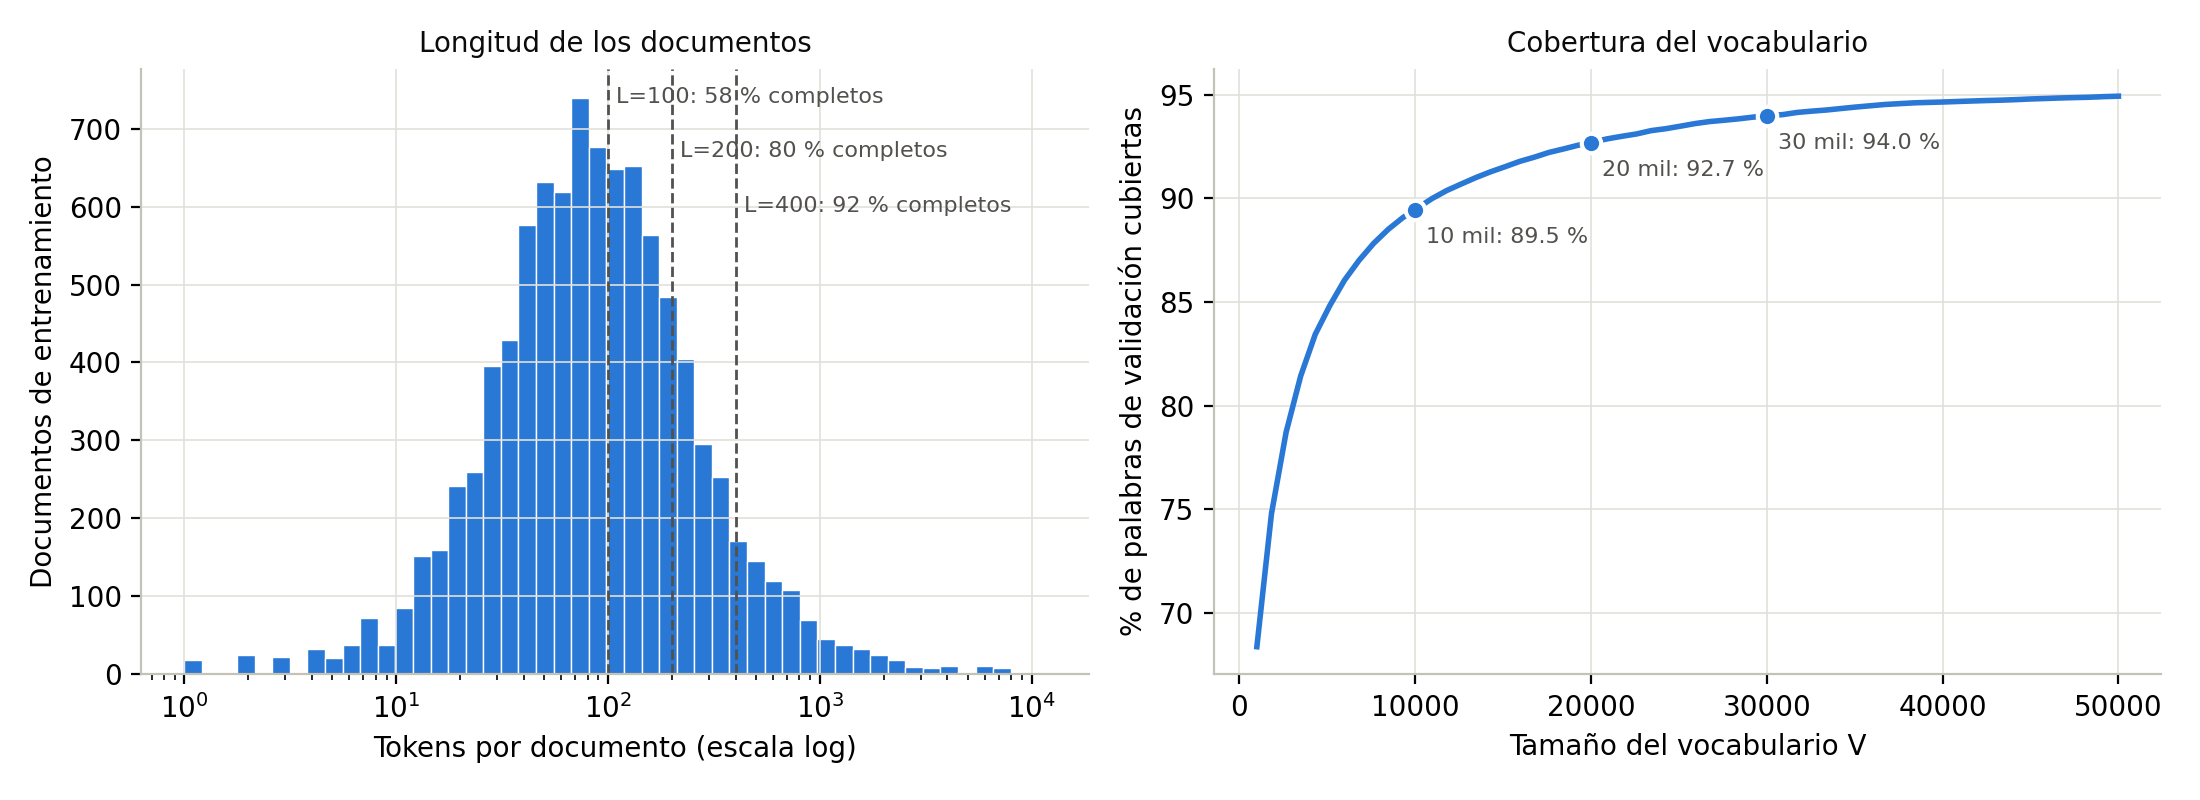
\includegraphics[width=\linewidth]{eda_longitudes_vocabulario.png}
\caption{Izquierda: longitud de los documentos de entrenamiento en tokens (escala logarítmica) con los tres valores de $L$ probados. Derecha: porcentaje de las palabras de validación que cubre el vocabulario de entrenamiento según su tamaño $V$.}
\label{fig:eda}
\end{figure}

\begin{table}[H]
\centering
\caption{Longitud de los documentos en tokens por partición y documentos vacíos tras la limpieza.}
\label{tab:eda_longitudes}
\small
\tablaancha{eda_longitudes}
\end{table}

\begin{table}[H]
\centering
\begin{minipage}{0.46\linewidth}
\centering
\caption{Documentos de entrenamiento que caben completos según $L$.}
\label{tab:eda_L}
\small
\tabla{eda_L}
\end{minipage}\hfill
\begin{minipage}{0.5\linewidth}
\centering
\caption{Cobertura del vocabulario en validación según $V$.}
\label{tab:eda_V}
\small
\resizebox{\linewidth}{!}{\tabla{eda_V}}
\end{minipage}
\end{table}

% ============================================================
\section{Fundamentos}\label{sec:fundamentos}
% ============================================================

\subsection{RNN sin memoria: SimpleRNN}

Una RNN simple (red de Elman~\cite{elman1990}) procesa la secuencia $x_1, \dots, x_T$ actualizando un estado oculto:
\begin{equation}
    h_t = \tanh\left(W_x x_t + W_h h_{t-1} + b\right),
\end{equation}
donde $x_t$ es el vector (embedding) de la palabra $t$. Para clasificar se usa el último estado $h_T$. Su capa recurrente tiene $h(d+h+1)$ parámetros, con $d$ la dimensión del embedding y $h$ el número de unidades.

El entrenamiento usa retropropagación a través del tiempo (BPTT): la red se ``desenrolla'' en los $T$ pasos y el gradiente de la pérdida con respecto a un paso lejano contiene el producto
\begin{equation}
    \frac{\partial h_T}{\partial h_t} = \prod_{k=t+1}^{T} \operatorname{diag}\left(1 - h_k^2\right) W_h ,
\end{equation}
cuya norma tiende a encogerse (o a crecer) exponencialmente con la distancia $T-t$~\cite{bengio1994,pascanu2013}. Este \textbf{desvanecimiento del gradiente} hace que la SimpleRNN aprenda con dificultad de las palabras que están lejos del final de la secuencia: por eso se le considera una red ``sin memoria'' de largo plazo, aunque tenga un estado oculto. El problema opuesto, la explosión del gradiente, se controla recortando su norma~\cite{pascanu2013}.

\subsection{RNN con memoria: LSTM}

La LSTM~\cite{hochreiter1997} agrega una celda de memoria $c_t$ y tres compuertas que deciden qué entra, qué se olvida y qué sale:
\begin{align}
    i_t &= \sigma(W_i x_t + U_i h_{t-1} + b_i), \qquad
    f_t = \sigma(W_f x_t + U_f h_{t-1} + b_f), \\
    o_t &= \sigma(W_o x_t + U_o h_{t-1} + b_o), \qquad
    g_t = \tanh(W_g x_t + U_g h_{t-1} + b_g), \\
    c_t &= f_t \odot c_{t-1} + i_t \odot g_t, \qquad h_t = o_t \odot \tanh(c_t).
\end{align}
La actualización de $c_t$ es una \textbf{suma}: entre un paso y el siguiente el gradiente se multiplica por la compuerta de olvido $f_t$ y no por una matriz, de modo que la información y el gradiente pueden atravesar muchos pasos sin desvanecerse~\cite{hochreiter1997,goodfellow2016}. El costo es tener cuatro transformaciones en lugar de una: la capa tiene $4h(d+h+1)$ parámetros.

% ============================================================
\section{Arquitecturas}\label{sec:arquitectura}
% ============================================================

Los dos modelos comparten el mismo esqueleto y solo cambia la capa recurrente, para que la diferencia entre ellos se deba a la memoria:
\begin{center}
\small
texto $\rightarrow$ \texttt{TextVectorization} $\rightarrow$ \texttt{Embedding}($V$, 100, \texttt{mask\_zero=True}) $\rightarrow$ \textbf{SimpleRNN} o \textbf{LSTM} ($h$ unidades) $\rightarrow$ \texttt{Dropout} $\rightarrow$ \texttt{Dense}(20, softmax)
\end{center}

\begin{table}[H]
\centering
\caption{Componentes de la arquitectura y su justificación.}
\label{tab:arquitectura}
\small
\begin{tabularx}{\linewidth}{>{\raggedright\arraybackslash}p{3.2cm} >{\raggedright\arraybackslash}p{3.6cm} X}
\toprule
\textbf{Componente} & \textbf{Valor} & \textbf{Justificación} \\
\midrule
RNN sin memoria & Capa \texttt{SimpleRNN} de Keras & Lo pide el enunciado; es la red de Elman~\cite{elman1990}. \\
RNN con memoria & Capa \texttt{LSTM} de Keras & El enunciado permite LSTM, GRU o Transformer; la LSTM tiene una celda de memoria explícita, que es lo que se quiere comparar~\cite{hochreiter1997}. \\
Embedding & 100 dimensiones, entrenado desde cero & Tamaño del ejemplo oficial de Keras con 20 Newsgroups~\cite{kerasglove}. \\
Unidades $h$ & 128 al inicio; se prueban 64 y 256 & Valor de partida; el final sale de validación (Sección~\ref{sec:ajuste}). \\
Salida & Último estado oculto $\rightarrow$ Dense(20, softmax) & Igual en ambos modelos. Softmax como en la Entrega~1: cada documento tiene una sola etiqueta entre 20. \\
Dropout & 0.3 después de la capa recurrente; se prueban 0.2 y 0.5 & La Entrega~1 usó 0.3--0.4; el valor final sale de validación. \\
Sin dropout recurrente & \texttt{recurrent\_dropout} $=0$ & Con \texttt{recurrent\_dropout} $>0$ la LSTM no puede usar su implementación rápida (cuDNN) en GPU~\cite{kerasdocs}. \\
\bottomrule
\end{tabularx}
\end{table}

Con $V=20\,000$, $d=100$, $h=128$ y 20 clases, la capa SimpleRNN tiene $128\,(100+128+1)=29\,312$ parámetros y la LSTM $4\times 29\,312 = 117\,248$; con el embedding ($2\,000\,000$) y la capa de salida ($2\,580$) los modelos completos suman $2\,031\,892$ y $2\,119\,828$ parámetros (verificado con \texttt{model.summary()}). Con las 256 unidades que se eligieron en el ajuste, la SimpleRNN final tiene $2\,096\,532$. Es decir, entre el $94\%$ y el $98\%$ de los parámetros está en el embedding. Como referencia, el MLP \textit{Tuned} de la Entrega~1 tiene $5\,256\,980$ parámetros.

% ============================================================
\section{Condiciones de entrenamiento}\label{sec:entrenamiento}
% ============================================================

\begin{table}[H]
\centering
\caption{Condiciones de entrenamiento y su justificación.}
\label{tab:condiciones}
\small
\begin{tabularx}{\linewidth}{>{\raggedright\arraybackslash}p{3.3cm} >{\raggedright\arraybackslash}p{4.8cm} X}
\toprule
\textbf{Elemento} & \textbf{Valor} & \textbf{Justificación} \\
\midrule
Optimizador & Adam, tasa de aprendizaje $10^{-3}$ & Igual que la Entrega~1. \\
Recorte del gradiente & \texttt{clipnorm=1.0} & Evita la explosión del gradiente, típica de las RNN~\cite{pascanu2013}. \\
Pérdida & Entropía cruzada categórica (\texttt{sparse}) & Igual que la Entrega~1. \\
Tamaño de lote & 64 & Igual que la Entrega~1. \\
Épocas & Máximo 30, con \texttt{EarlyStopping} (val\_loss, paciencia 4) & Igual que la Entrega~1; el máximo sube de 20--25 a 30 porque una RNN puede necesitar más épocas. \\
Tasa de aprendizaje & \texttt{ReduceLROnPlateau} ($\times 0.5$, paciencia 2) & Igual que la Entrega~1. \\
Pesos finales & Los de la época con menor val\_loss & \texttt{ModelCheckpoint} con \texttt{save\_best\_only}. \\
Semillas & 42 durante el ajuste; 1, 7 y 123 solo con la configuración final & Se conserva la de mejor F1 macro de validación (la 42) y se reportan todas (Sección~\ref{sec:semillas}). \\
Entorno & Google Colab con GPU NVIDIA Tesla T4; TensorFlow 2.21.0, Keras 3.13.2, scikit-learn 1.6.1, Python 3.13 & Registrado automáticamente en cada corrida (\texttt{results/e2/runs/*/config.json}). \\
\bottomrule
\end{tabularx}
\end{table}

\subsection{Uso de las semillas}\label{sec:semillas}

En la Entrega~1 los dos MLP se re-entrenaron con cuatro semillas (42, 1, 7 y 123), y en la retroalimentación de esa entrega la profesora señaló que no era adecuado variar la semilla. En esta entrega se mantuvo ese antecedente, pero con un uso acotado y declarado desde el principio:
\begin{enumerate}
    \item Todo el ajuste de la Sección~\ref{sec:ajuste} se hizo con una sola semilla fija, la 42, la misma de la Entrega~1.
    \item Solo con la configuración final ya fijada, cada red se entrenó otras tres veces, con las semillas 1, 7 y 123. No cambió nada más: ni los datos, ni la partición, ni los hiperparámetros.
    \item Entre las cuatro, se escogió como modelo final de cada red la semilla con mejor F1 macro de validación. En las dos RNN fue la 42 (Tabla~\ref{tab:semillas}); sus resultados son los de las tablas principales y los que usa la demostración. También en el MLP de referencia la 42 tuvo la mejor exactitud de validación ($74.03\%$). La elección se hizo con validación: el conjunto de prueba no intervino.
    \item Los resultados de las otras tres semillas no se descartan: se reportan todos, con su media y su desviación estándar.
\end{enumerate}

Se volvió a variar la semilla por dos razones. La primera es que las RNN dependen mucho más de la inicialización que el MLP: con la misma configuración, el F1 macro de validación de la LSTM fue de $47.16\%$ a $55.62\%$ según la semilla, y el de la SimpleRNN de $21.25\%$ a $26.43\%$, mientras que el MLP apenas cambia (su F1 macro de prueba va de $66.19\%$ a $66.58\%$). Con una sola semilla no se podría saber si la diferencia entre las dos redes se debe a la memoria o a una inicialización afortunada; con cuatro se comprueba que no: el peor resultado de la LSTM en prueba ($43.58\%$ de F1 macro) supera con holgura al mejor de la SimpleRNN ($23.97\%$). La segunda razón es que escoger la mejor semilla hace que la cifra reportada sea optimista, más aún porque el ajuste se hizo con la 42; por eso, junto a ella, se reporta siempre la media de las cuatro, que es la estimación más conservadora.

% ============================================================
\section{Ajuste de parámetros}\label{sec:ajuste}
% ============================================================

El ajuste se hizo igual para los dos modelos y únicamente con el conjunto de validación:
\begin{enumerate}
    \item Se entrena la configuración base (Secciones~\ref{sec:arquitectura} y~\ref{sec:entrenamiento}) con $L=200$ y la semilla 42, que queda fija durante todo el ajuste.
    \item Se prueban los parámetros \textbf{uno a la vez}, en este orden: longitud $L \in \{100, 200, 400\}$, unidades $\in \{64, 128, 256\}$, dropout $\in \{0.2, 0.3, 0.5\}$ y tasa de aprendizaje $\in \{10^{-3}, 5\times 10^{-4}\}$. Cada paso parte de la mejor configuración del paso anterior.
    \item Un cambio se adopta solo si mejora el F1 macro de validación en más de $0.5$ puntos. Por debajo de ese umbral la diferencia se trata como ruido: en la Entrega~1 la exactitud varió entre $\pm 0.3$ y $\pm 0.9$ puntos solo por cambiar la semilla.
    \item La configuración final de cada modelo se entrena con cuatro semillas (Sección~\ref{sec:semillas}), y cada modelo resultante se evalúa \textbf{una sola vez} en el conjunto de prueba. La prueba no se usa para escoger nada.
\end{enumerate}
Cambiar un parámetro a la vez permite atribuir cada mejora a un parámetro concreto, algo que la Entrega~1 no pudo hacer porque cambió cinco a la vez. Las Tablas~\ref{tab:ajuste_simple} y~\ref{tab:ajuste_lstm} muestran todas las pruebas; la Figura~\ref{fig:ajuste} las resume.

\begin{table}[H]
\centering
\caption{Ajuste de la SimpleRNN (F1 macro y exactitud en validación). En negrita y con $\checkmark$, el valor elegido en cada paso.}
\label{tab:ajuste_simple}
\small
\tablaancha{ajuste_simple}
\end{table}

\begin{table}[H]
\centering
\caption{Ajuste de la LSTM, con el mismo formato de la Tabla~\ref{tab:ajuste_simple}.}
\label{tab:ajuste_lstm}
\small
\tablaancha{ajuste_lstm}
\end{table}

\begin{figure}[H]
\centering
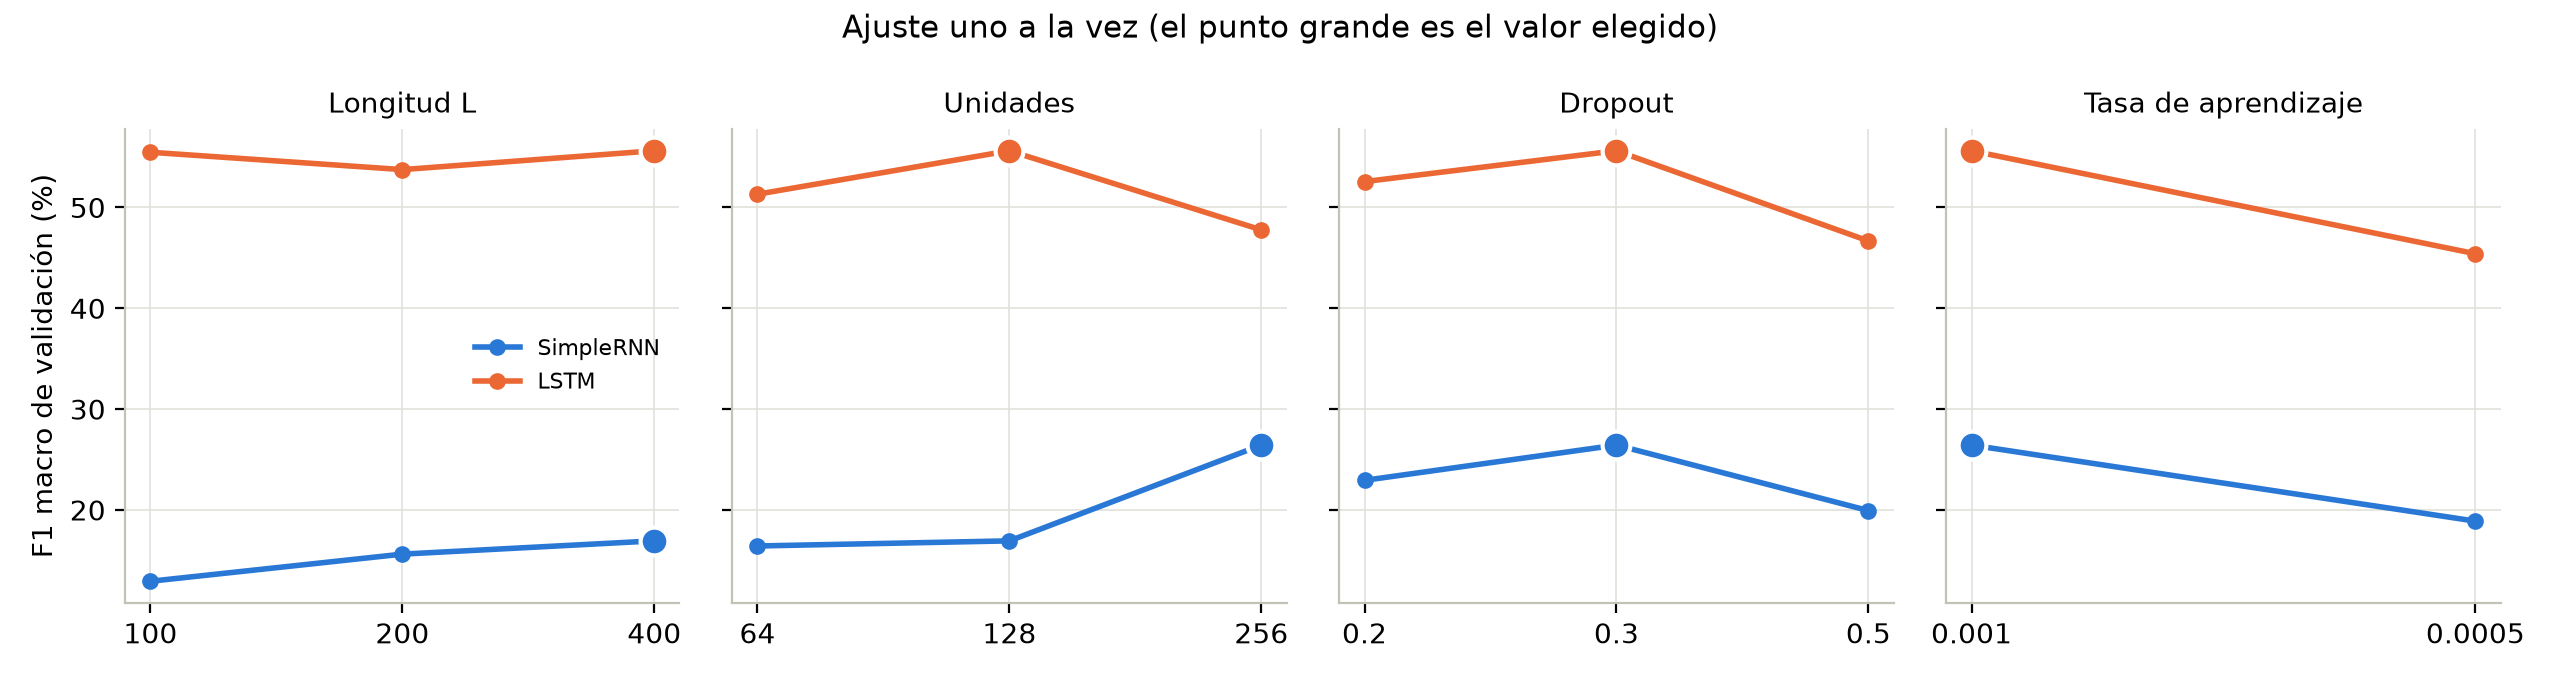
\includegraphics[width=\linewidth]{ajuste.png}
\caption{F1 macro de validación en cada paso del ajuste. El punto grande marca el valor elegido.}
\label{fig:ajuste}
\end{figure}

\textbf{SimpleRNN.} Dos cambios superaron el umbral: $L=400$ (+1.31 puntos de F1 macro) y, sobre todo, 256 unidades (+9.50 puntos). Con 64 y 128 unidades la red memorizó el conjunto de entrenamiento en 6 o 7 épocas (exactitud de entrenamiento entre $92\%$ y $96\%$) mientras la exactitud de validación se quedaba entre $15\%$ y $18\%$ desde la segunda época. Con 256 unidades la dinámica fue otra: pasó varias épocas cerca del azar y después aprendió algo que generaliza mejor (Sección~\ref{sec:curvas}). Ni el dropout ni la tasa de aprendizaje mejoraron el valor de partida. En total, el F1 macro de validación subió de $15.62\%$ a $26.43\%$ (Tabla~\ref{tab:base_ajustado}).

\textbf{LSTM.} Solo se adoptó $L=400$ (+1.87 puntos). Con $L=100$ el resultado fue casi igual ($55.47\%$ frente a $55.62\%$) en la mitad del tiempo por época. Las demás alternativas empeoraron entre 3 y 10 puntos: con 256 unidades o con dropout de 0.5 la pérdida de validación llegó a su mínimo antes (época 6) y con un F1 menor, y con 64 unidades o dropout de 0.2 la red rindió algo menos. El F1 macro de validación pasó de $53.75\%$ a $55.62\%$: la configuración de partida ya estaba cerca de la mejor que permite esta búsqueda.

\textbf{Dos precauciones al leer el ajuste.} Primero, el umbral de 0.5 puntos se fijó con la variación del MLP en la Entrega~1, pero las RNN resultaron mucho más sensibles a la semilla. Al repetir las configuraciones finales con cuatro semillas, el F1 macro de validación varió $\pm 2.3$ puntos en la SimpleRNN y $\pm 4.2$ en la LSTM (en prueba, $\pm 2.4$ y $\pm 3.0$; Tabla~\ref{tab:semillas}). Por eso las diferencias de uno o dos puntos de las Tablas~\ref{tab:ajuste_simple} y~\ref{tab:ajuste_lstm} no son concluyentes; sí lo son las grandes, como las 256 unidades de la SimpleRNN (+9.5) o las caídas de la LSTM con dropout de 0.5 ($-8.9$) y con 256 unidades ($-7.9$). Hacerlo mejor exigiría repetir cada prueba con varias semillas, lo que multiplica el costo del ajuste. Segundo, la parada temprana elige la época con menor pérdida de validación, mientras que el ajuste compara el F1 macro, y los dos criterios no siempre coinciden: con tasa $5\times10^{-4}$ la LSTM logró la menor pérdida de validación de todo su ajuste (1.591), pero en esa época su exactitud de validación era de $47\%$ y seguía subiendo (llegó a $53\%$ cuando la parada temprana detuvo el entrenamiento). El resultado de esa tasa está, por tanto, subestimado.

\begin{table}[H]
\centering
\caption{Configuración base frente a configuración ajustada (resultados de validación).}
\label{tab:base_ajustado}
\small
\tablaancha{base_vs_ajustado}
\end{table}

% ============================================================
\section{Resultados y análisis}\label{sec:resultados}
% ============================================================

\subsection{Resultados en el conjunto de prueba}

La Tabla~\ref{tab:final} reúne los resultados de prueba de los dos modelos ajustados y del MLP. Para que la comparación con la Entrega~1 sea justa, el MLP \textit{Tuned} se re-entrenó en el mismo entorno y con la misma partición: obtuvo $67.74\%$ de exactitud, frente a $68.03\%$ en la Entrega~1, una diferencia que cabe dentro de su variación entre semillas (Tabla~\ref{tab:semillas}).

\begin{table}[H]
\centering
\caption{Resultados en el conjunto de prueba (7\,532 documentos) con la semilla 42, la de mejor F1 macro de validación entre las cuatro probadas (Sección~\ref{sec:semillas}). Exactitud, F1 macro, precisión y exhaustividad en \%; las tres últimas son promedios macro. Las dos primeras filas se copian de los archivos de resultados de la Entrega~1.}
\label{tab:final}
\small
\tablaancha{final}
\end{table}

\begin{figure}[H]
\centering
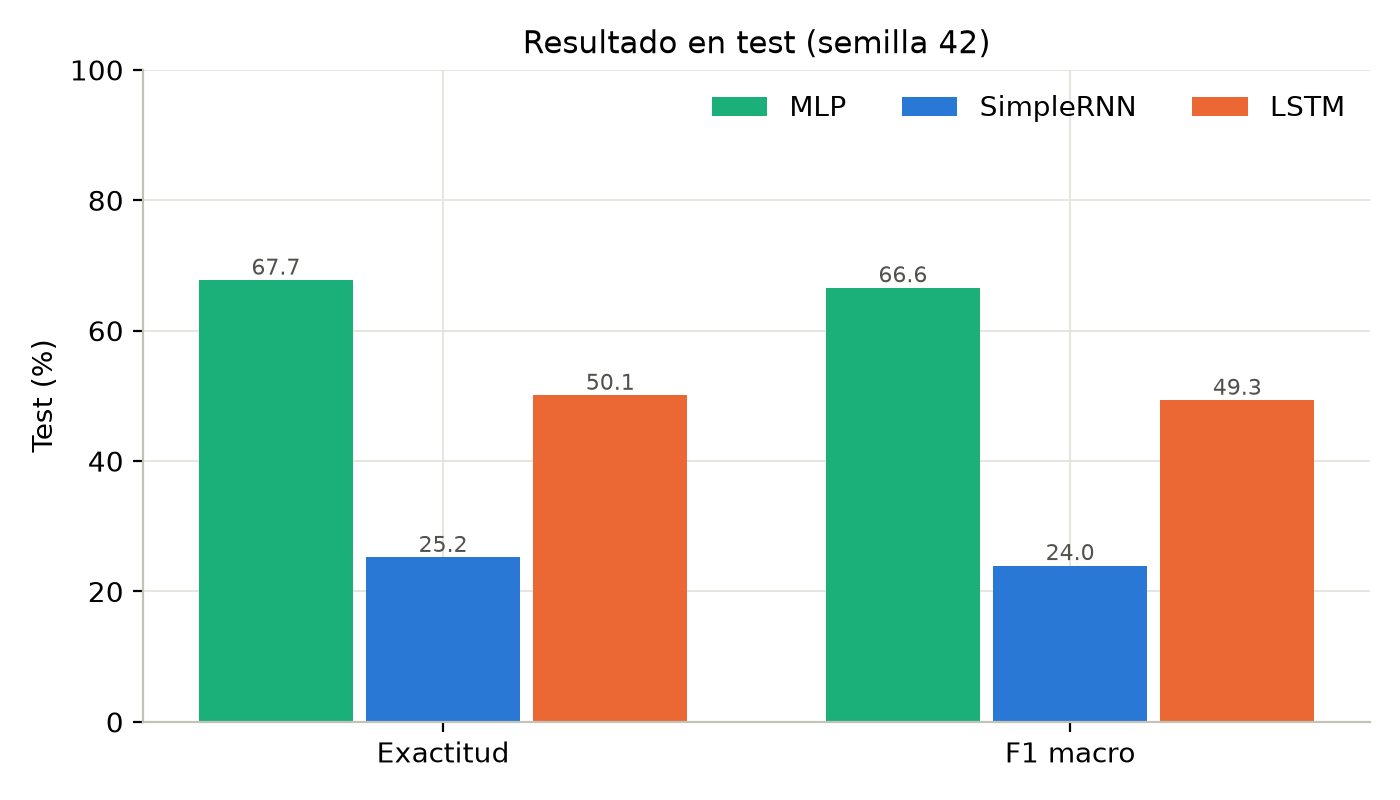
\includegraphics[width=0.78\linewidth]{comparacion_final.png}
\caption{Exactitud y F1 macro en prueba de los tres modelos (semilla 42).}
\label{fig:comparacion_final}
\end{figure}

La LSTM duplica a la SimpleRNN en las cuatro métricas: $50.08\%$ frente a $25.21\%$ de exactitud y $49.32\%$ frente a $23.97\%$ de F1 macro. Con 20 clases, clasificar al azar daría un $5\%$, así que la SimpleRNN sí aprendió algo, pero poco. El MLP supera a las dos: queda 17.7 puntos de exactitud por encima de la LSTM y 42.5 por encima de la SimpleRNN.

De validación a prueba, la exactitud baja 6.3 puntos tanto en la LSTM ($56.36\% \rightarrow 50.08\%$) como en el MLP ($74.03\% \rightarrow 67.74\%$). Como la caída es la misma en dos modelos muy distintos, se explica mejor por la partición que por un sobreajuste a la validación: el conjunto de prueba de 20 Newsgroups contiene mensajes publicados después de los de entrenamiento~\cite{sklearn20ng}, y los temas y el vocabulario cambian con el tiempo.

\textbf{Resultados por semilla.} La Tabla~\ref{tab:semillas} muestra el F1 macro de validación y de prueba de las cuatro semillas. La 42, escogida por validación (Sección~\ref{sec:semillas}), es la que aparece en las tablas y figuras anteriores. La diferencia entre la LSTM y la SimpleRNN, 25.4 puntos de F1 macro de prueba en promedio, es unas diez veces mayor que la desviación estándar de cualquiera de las dos, así que no depende de la semilla. Las RNN varían entre 14 y 17 veces más que el MLP ($\pm 2.4$ y $\pm 3.0$ puntos de F1 macro de prueba, frente a $\pm 0.17$). La semilla 42 también fue la mejor de las cuatro en prueba para las dos RNN, algo esperable porque el ajuste se hizo con ella; el promedio de las cuatro ($46.1\%$ de F1 macro para la LSTM y $20.7\%$ para la SimpleRNN) es la estimación más conservadora.

\begin{table}[H]
\centering
\caption{F1 macro (\%) de cada semilla con la configuración final, en validación y en prueba. En negrita, la semilla escogida como modelo final (la de mejor F1 macro de validación); la última fila es la media $\pm$ desviación estándar de las cuatro. Del MLP solo se guardó el F1 de prueba.}
\label{tab:semillas}
\small
\tablaancha{por_semilla}
\end{table}

\subsection{Curvas de entrenamiento}\label{sec:curvas}

\begin{figure}[H]
\centering
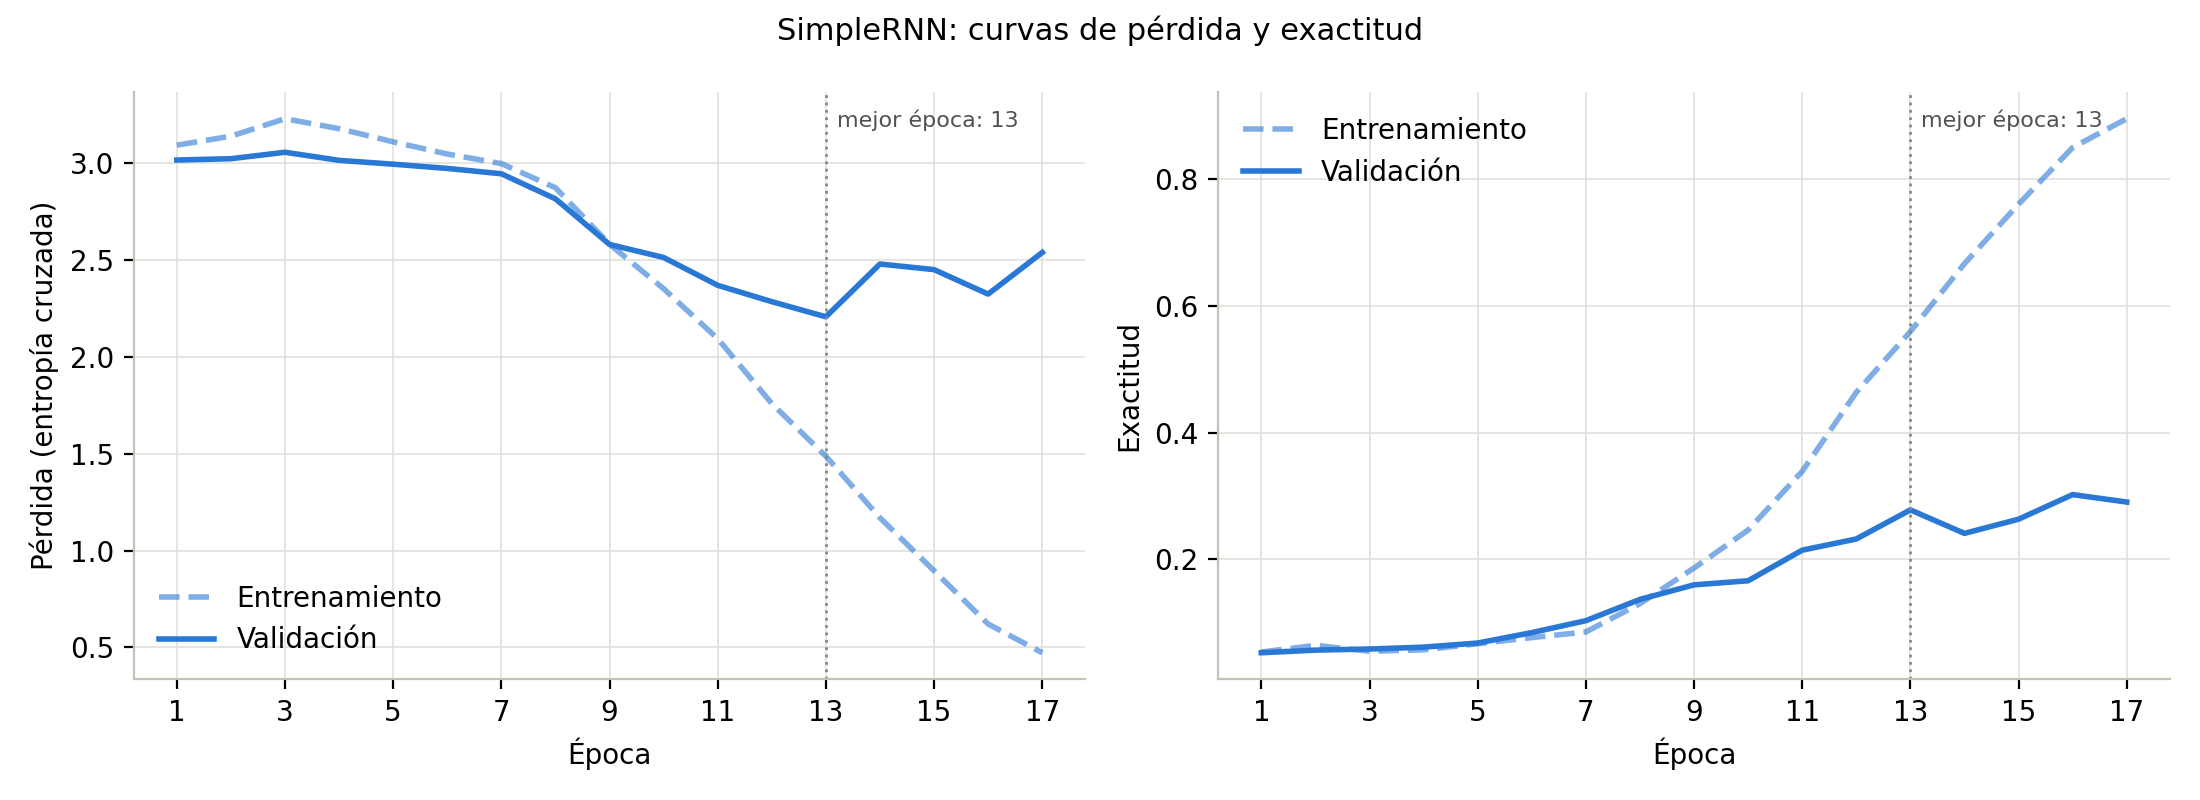
\includegraphics[width=\linewidth]{curvas_simple.png}\\[4pt]
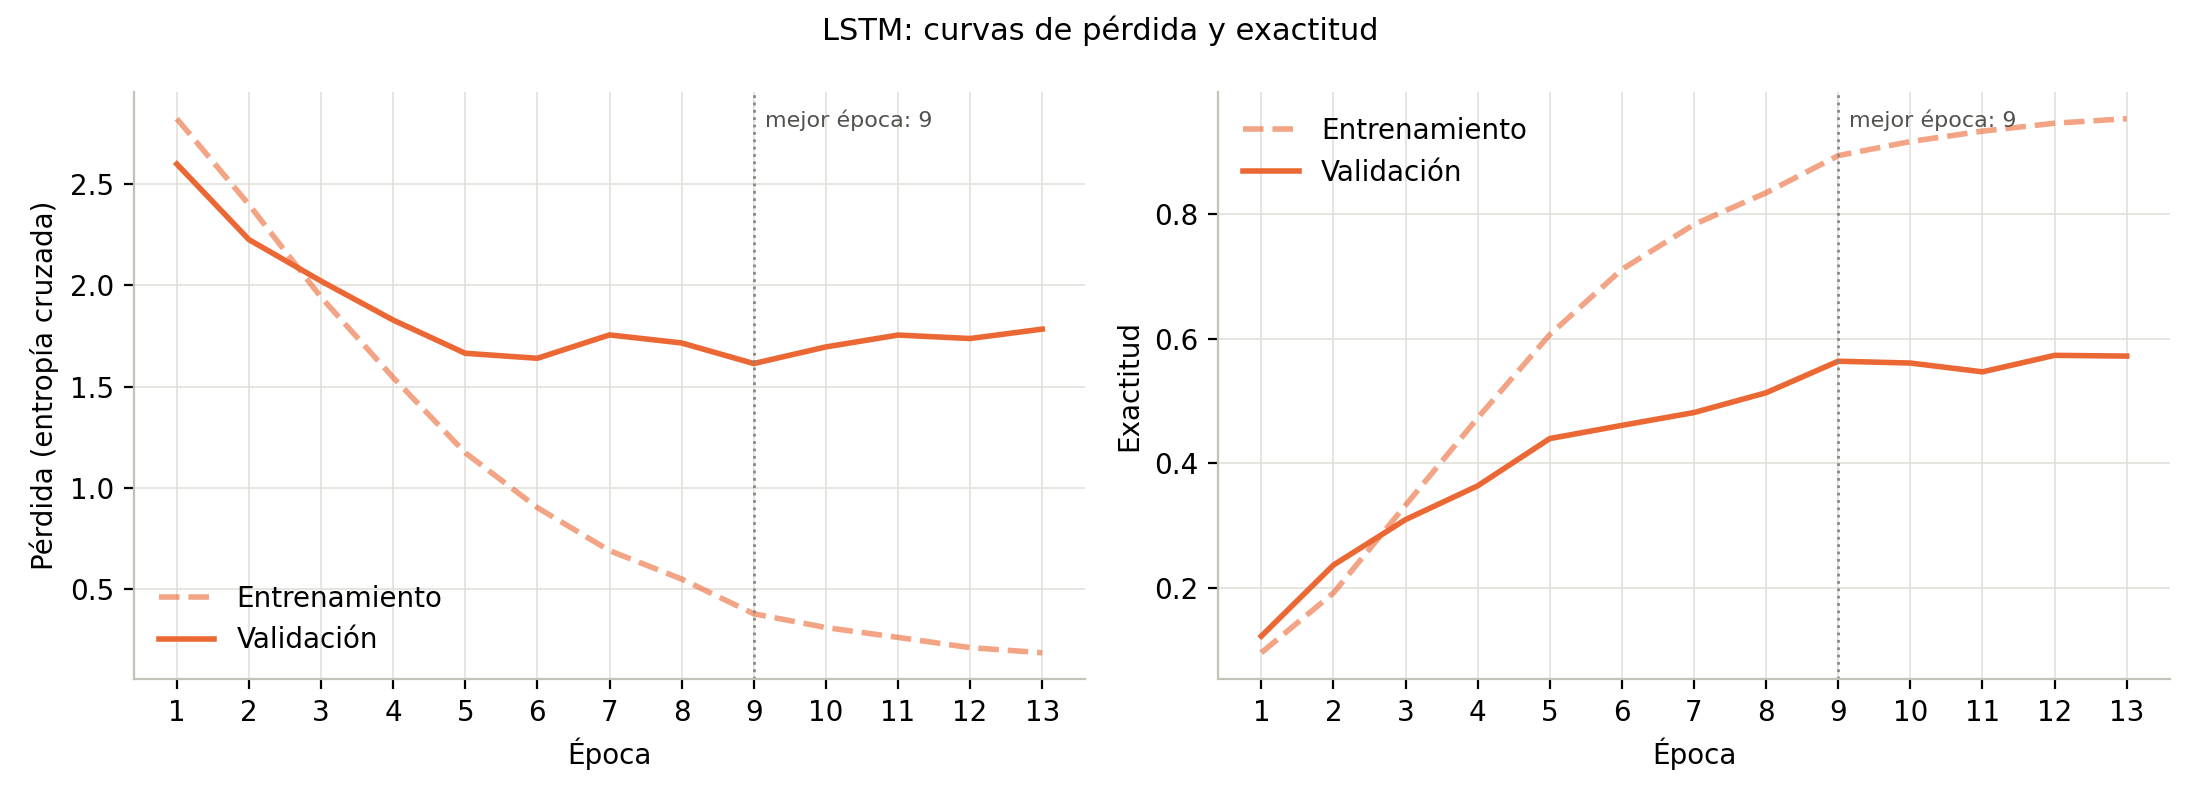
\includegraphics[width=\linewidth]{curvas_lstm.png}
\caption{Pérdida y exactitud por época de la SimpleRNN (arriba) y de la LSTM (abajo) con la configuración final. Línea discontinua: entrenamiento; continua: validación. La línea punteada marca la época cuyos pesos se conservan.}
\label{fig:curvas}
\end{figure}

La Figura~\ref{fig:curvas} muestra dos comportamientos muy distintos. La \textbf{SimpleRNN} pasa sus primeras siete épocas cerca del azar: la exactitud no supera el $10\%$ y la pérdida se queda alrededor de 3.0, que es $\ln 20$, el valor que se obtiene al dar la misma probabilidad a las 20 clases. Solo desde la octava época empieza a aprender, y entonces sobreajusta rápido: la exactitud de entrenamiento llega al $90\%$ mientras la de validación se queda alrededor del $30\%$. Las otras tres semillas repiten el patrón, con entre 3 y 6 épocas iniciales cerca del azar. La \textbf{LSTM}, en cambio, aprende desde la primera época: la exactitud de validación sube de $12\%$ a $56\%$ hasta la época 9, donde la pérdida de validación llega a su mínimo; después la red sigue mejorando en entrenamiento (hasta $95\%$) sin mejorar en validación, y la parada temprana la detiene en la época 13 con los pesos de la época 9. La Figura~\ref{fig:comparacion_validacion} pone las dos curvas de validación lado a lado.

Las dos redes sobreajustan, lo cual es esperable: tienen unos dos millones de parámetros, casi todos en el embedding, y solo 9\,616 documentos para aprenderlos desde cero. El MLP de la Entrega~1 también sobreajusta (llega a $96\%$ en entrenamiento mientras la validación se queda en $73$--$74\%$), pero parte de vectores TF-IDF que ya resumen el documento completo.

\begin{figure}[H]
\centering
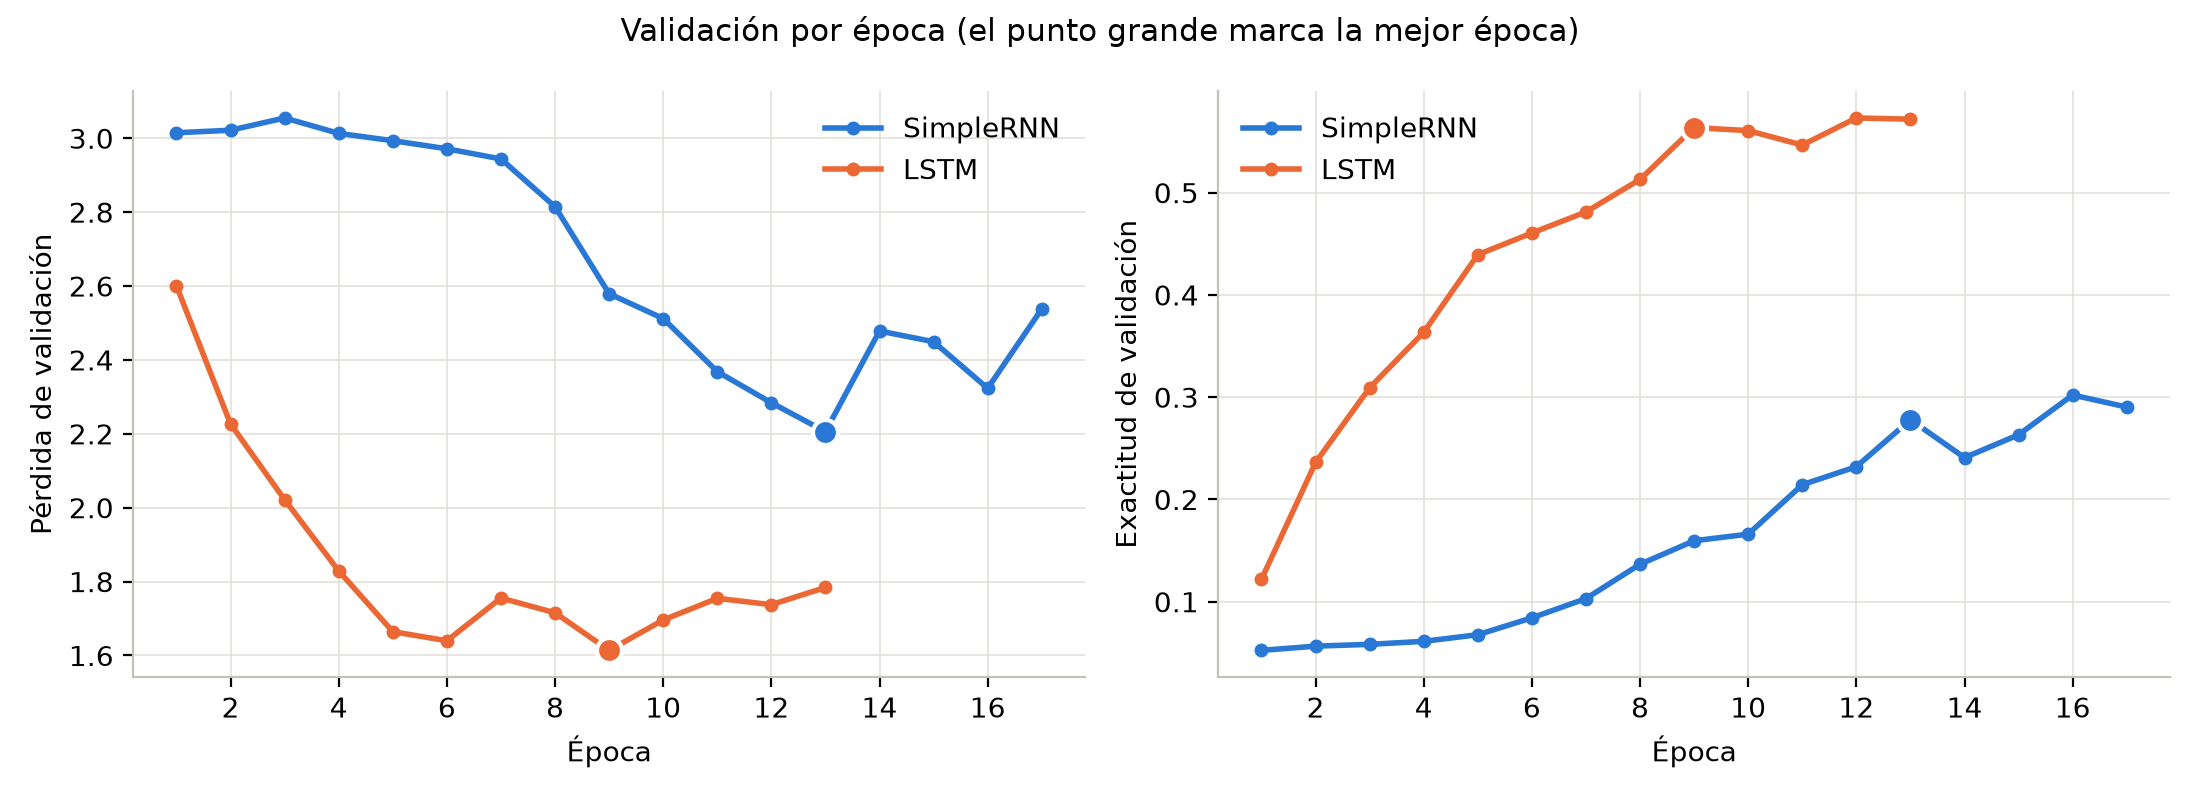
\includegraphics[width=\linewidth]{comparacion_validacion.png}
\caption{Pérdida y exactitud de validación por época de las dos RNN finales. El punto grande marca la época cuyos pesos se conservan.}
\label{fig:comparacion_validacion}
\end{figure}

\subsection{Memoria: SimpleRNN frente a LSTM}\label{sec:memoria}

Según la Sección~\ref{sec:fundamentos}, la SimpleRNN debería aprender con dificultad de las palabras lejanas al final de la secuencia, porque el gradiente que llega a ellas se multiplica por $W_h$ en cada paso, mientras que la celda de la LSTM deja pasar la información y el gradiente a través de una suma. Además de la meseta inicial de la SimpleRNN, otras dos mediciones permiten comprobarlo: la prueba de esta sección y el análisis por longitud de la siguiente.

\textbf{Prueba de memoria con distancia controlada.} Se escribieron 8 frases con un tema claro (por ejemplo, ``\textit{The engine needs a new oil filter and spark plugs for better mileage}'' para \clase{rec.autos}) y a cada una se le agregaron $k$ palabras de relleno sin tema \emph{después} de la frase, con tres textos de relleno distintos ($8 \times 3 = 24$ casos por distancia; script \texttt{memoria\_e2.py}). Como las RNN clasifican con su último estado, el tema tiene que atravesar $k$ pasos para llegar a la salida. La Figura~\ref{fig:memoria} y la Tabla~\ref{tab:memoria} muestran el resultado:
\begin{itemize}
    \item el \textbf{MLP} no depende del orden: acierta los 24 casos a cualquier distancia, y la probabilidad de la clase correcta solo baja lentamente porque el relleno diluye el peso TF-IDF de las palabras del tema;
    \item la \textbf{LSTM} acierta todos los casos con hasta 10 palabras de relleno y el $83\%$ con 25, pero con 50 ya solo acierta el $17\%$;
    \item la \textbf{SimpleRNN} parte de un $50\%$ de aciertos sin relleno, baja al $33\%$ con 10 palabras y al $4\%$ con 50; desde ahí su probabilidad para la clase correcta queda en el nivel del azar.
\end{itemize}
La memoria de la LSTM es, entonces, más larga que la de la SimpleRNN, pero no ilimitada: unas decenas de palabras sin relación bastan para que su estado olvide el tema. En los documentos reales el texto que sigue a una frase suele tratar del mismo tema, así que esta prueba es más exigente que la clasificación real; aun así, ayuda a entender por qué las RNN pierden frente al MLP en los documentos largos.

\begin{figure}[H]
\centering
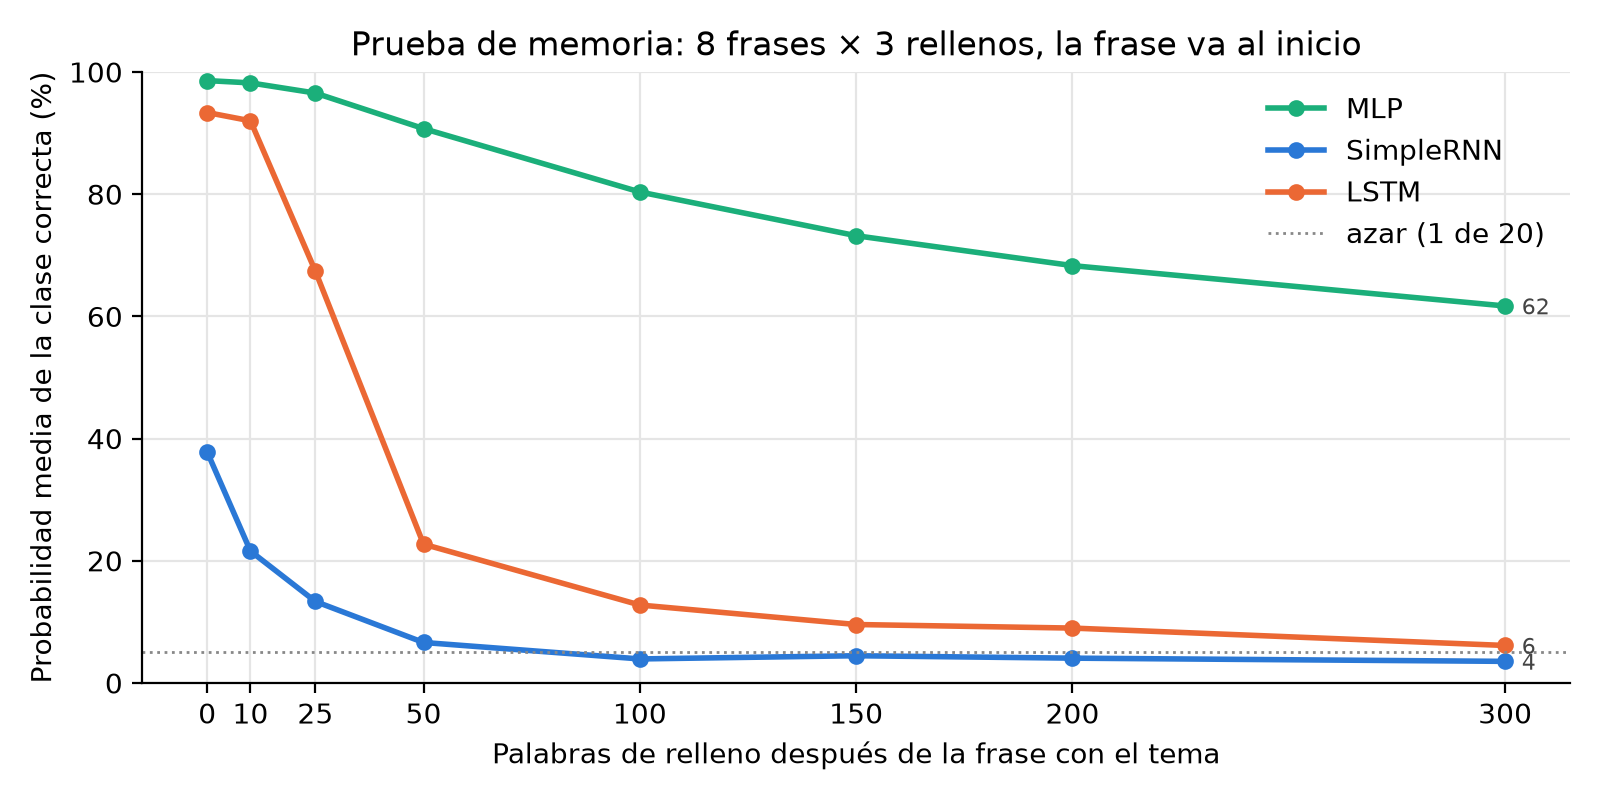
\includegraphics[width=0.85\linewidth]{memoria.png}
\caption{Prueba de memoria: probabilidad media de la clase correcta según el número de palabras de relleno que siguen a la frase con el tema (24 casos por distancia).}
\label{fig:memoria}
\end{figure}

\begin{table}[H]
\centering
\caption{Prueba de memoria: porcentaje de los 24 casos en que la clase correcta es la primera opción.}
\label{tab:memoria}
\small
\tabla{memoria}
\end{table}

\textbf{Costo de entrenamiento.} Aunque tiene cuatro veces más parámetros recurrentes por unidad, la LSTM fue más rápida en GPU: 3.8 segundos por época, frente a 6.9 de la SimpleRNN final y 6.5 de la SimpleRNN con 128 unidades (Tabla~\ref{tab:ajuste_simple}). La razón es la implementación: la capa \texttt{LSTM} de Keras usa el núcleo de cuDNN cuando se cumplen sus condiciones (entre ellas, \texttt{recurrent\_dropout} $=0$ y relleno a la derecha), mientras que \texttt{SimpleRNN} no tiene esa versión y se ejecuta paso a paso~\cite{kerasdocs}. El entrenamiento final tomó 49 segundos en la LSTM, 117 en la SimpleRNN y 14 en el MLP.

\subsection{Exactitud según la longitud del documento}

Para ver dónde pierden las RNN, los documentos de prueba se dividieron en cuatro grupos según los cuartiles de longitud del conjunto de entrenamiento (Tabla~\ref{tab:longitud} y Figura~\ref{fig:longitud}).

\begin{table}[H]
\centering
\caption{Exactitud en prueba (\%) de cada modelo por grupo de longitud. Los límites son los cuartiles de longitud del conjunto de entrenamiento; los documentos truncados son los que superan $L=400$ tokens.}
\label{tab:longitud}
\small
\tablaancha{longitud}
\end{table}

\begin{figure}[H]
\centering
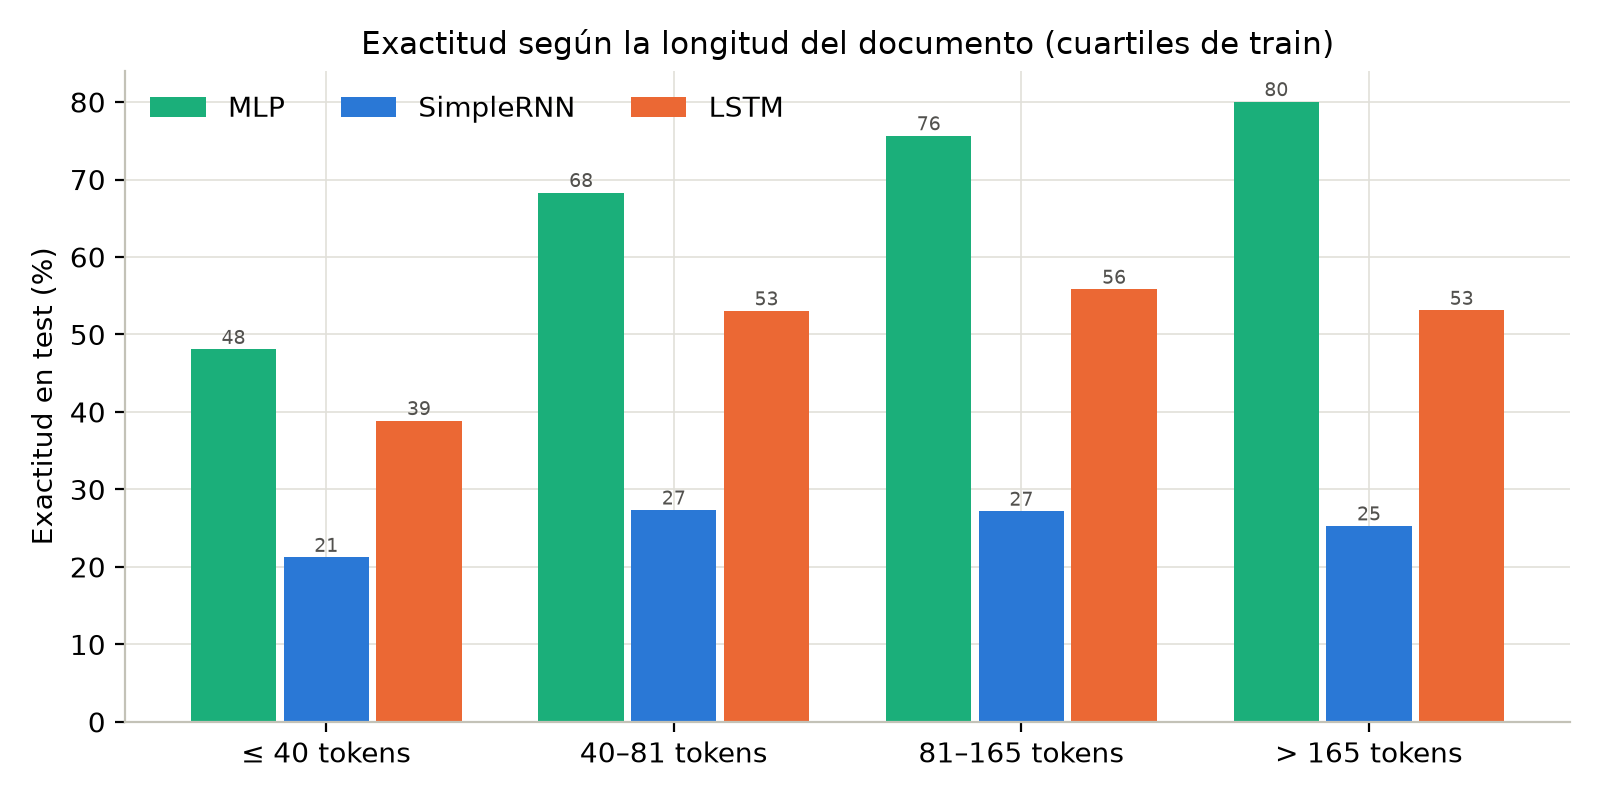
\includegraphics[width=0.85\linewidth]{longitud.png}
\caption{Exactitud en prueba según la longitud del documento.}
\label{fig:longitud}
\end{figure}

\begin{itemize}
    \item El \textbf{MLP} mejora siempre con la longitud, de $48.1\%$ en los documentos de hasta 40 tokens a $80.0\%$ en los de más de 165: más palabras son más evidencia para TF-IDF, que ve el documento completo.
    \item La \textbf{LSTM} mejora de $38.9\%$ a $55.8\%$ hasta los 165 tokens y luego baja un poco ($53.1\%$) en los documentos largos, donde el $31\%$ se trunca y el resto obliga a llevar la información a lo largo de cientos de pasos.
    \item La \textbf{SimpleRNN} se mantiene plana, entre $21\%$ y $27\%$ en todos los grupos: más texto no la ayuda, lo que concuerda con una red que en la práctica solo aprovecha la parte final de la secuencia.
\end{itemize}
La distancia entre el MLP y la LSTM crece con la longitud: es de 9.2 puntos en los documentos cortos y de 26.9 en los largos. La desventaja de las RNN se concentra en los documentos largos, en los que TF-IDF acumula la evidencia de todas las palabras y la red tiene que resumir cientos de pasos en un solo vector de estado de 128 números.

\subsection{Errores por clase}

\begin{figure}[H]
\centering
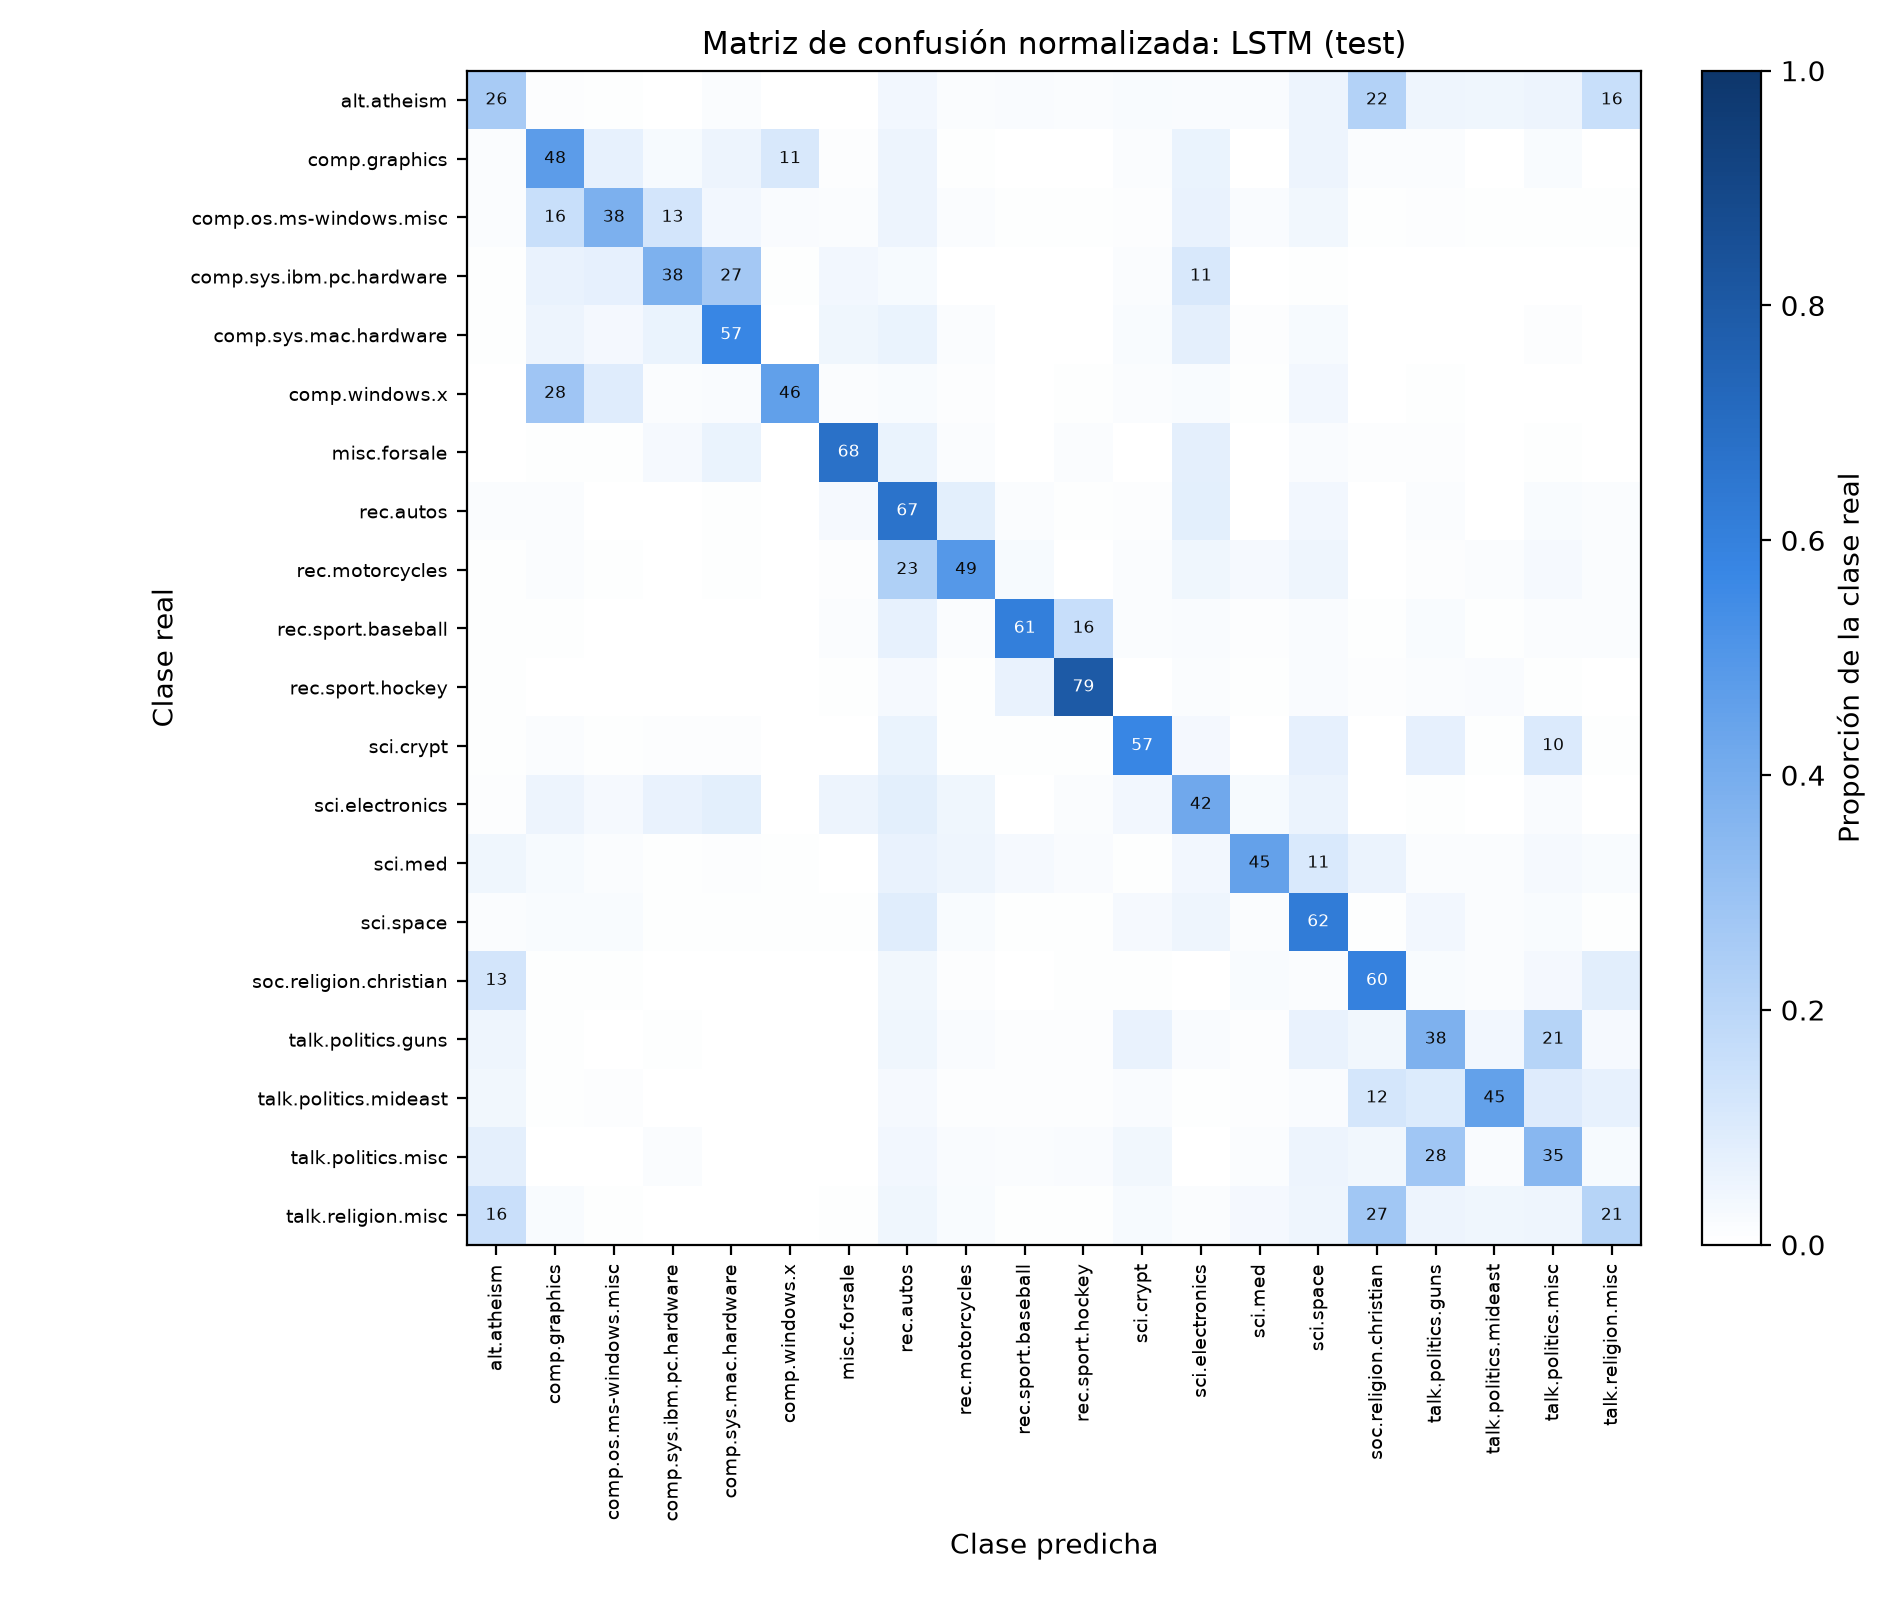
\includegraphics[width=0.88\linewidth]{confusion_mejor.png}
\caption{Matriz de confusión de la LSTM en prueba, normalizada por la clase real. Se rotulan las celdas de al menos $10\%$.}
\label{fig:confusion}
\end{figure}

La matriz de confusión de la LSTM (Figura~\ref{fig:confusion}) concentra los errores en grupos de la misma familia, que comparten vocabulario: \clase{comp.windows.x} se confunde con \clase{comp.graphics} en el $28\%$ de los casos, \clase{talk.politics.misc} con \clase{talk.politics.guns} ($28\%$), \clase{talk.religion.misc} con \clase{soc.religion.christian} ($27\%$), \clase{comp.sys.ibm.pc.hardware} con \clase{comp.sys.mac.hardware} ($27\%$) y \clase{rec.motorcycles} con \clase{rec.autos} ($23\%$). Las clases más difíciles coinciden en el MLP y en la LSTM (Tabla~\ref{tab:por_clase} del Anexo): \clase{talk.religion.misc}, \clase{alt.atheism} y \clase{talk.politics.misc} tienen el F1 más bajo en los dos modelos. Las mejores de la LSTM son \clase{rec.sport.hockey} ($76.1\%$), \clase{misc.forsale} ($70.2\%$) y \clase{rec.sport.baseball} ($67.0\%$).

\subsection{Comparación con el MLP de la Entrega~1}

Ninguna de las dos RNN alcanzó al MLP con TF-IDF. Los resultados anteriores apuntan a cuatro razones:
\begin{enumerate}
    \item \textbf{Pocos datos para un modelo de secuencia.} Con $S/W \approx 119$, muy por debajo del umbral de 1\,500 (Sección~\ref{sec:datos}), la literatura anticipa que un MLP sobre bolsa de palabras rinda igual o mejor~\cite{googletext,chollet2021deep}. Las RNN deben aprender desde cero un embedding de dos millones de parámetros con 9\,616 documentos, y sobreajustan pronto (Figura~\ref{fig:curvas}).
    \item \textbf{El tema depende más de las palabras que de su orden.} En la demostración (Sección~\ref{sec:demo}), intercambiar ``doctor'' y ``patient'' solo cambia la probabilidad de \clase{sci.med} de la LSTM de $99.04\%$ a $98.98\%$: la red sí lee el orden, pero el tema no cambia. Lo que aporta una RNN, el orden, importa poco en esta tarea.
    \item \textbf{Memoria limitada y truncamiento.} El MLP ve el documento completo; las RNN ven como máximo 400 tokens, deben resumirlos en un solo vector y su memoria se agota en unas decenas de palabras (Figura~\ref{fig:memoria}). Por eso la diferencia crece con la longitud del documento (Figura~\ref{fig:longitud}).
    \item \textbf{Costo.} El MLP también es el más barato: 2.0 segundos por época en la misma GPU, frente a 3.8 de la LSTM y 6.9 de la SimpleRNN.
\end{enumerate}

% ============================================================
\section{Demostración ejecutable}\label{sec:demo}
% ============================================================

El script \texttt{demo\_e2.py} carga los tres modelos guardados (el MLP \textit{Tuned} de la Entrega~1 re-entrenado, la SimpleRNN y la LSTM) y muestra, para un texto en inglés, las tres clases más probables según cada uno. Funciona sin conexión y sin descargar el conjunto de datos: usa los pesos y el vocabulario guardados en \texttt{models/e2/} y el mismo preprocesamiento del entrenamiento (se comprobó que sus probabilidades coinciden con las de la evaluación). Se ejecuta de tres formas:
\begin{center}
\texttt{python demo\_e2.py --run-samples} \quad\textbar\quad \texttt{python demo\_e2.py --text "..."} \quad\textbar\quad \texttt{python demo\_e2.py}
\end{center}
La primera corre los casos preparados para la sustentación, la segunda clasifica el texto que se le pase y la tercera abre un modo interactivo. El notebook \nolinkurl{notebooks/Demo_Entrega2_Colab.ipynb} hace lo mismo en Google Colab, sin instalar nada. La Tabla~\ref{tab:demo} resume los casos preparados; los cinco primeros son los de la demostración de la Entrega~1.

\begin{table}[H]
\centering
\caption{Casos de la demostración: clase más probable según cada modelo (probabilidad en \% entre paréntesis). En negrita, las respuestas que coinciden con la clase esperada; los casos mixtos no tienen una sola respuesta correcta.}
\label{tab:demo}
\scriptsize
\begin{tabularx}{\linewidth}{>{\raggedright\arraybackslash}X >{\raggedright\arraybackslash}p{2.15cm} >{\raggedright\arraybackslash}p{2.65cm} >{\raggedright\arraybackslash}p{2.65cm} >{\raggedright\arraybackslash}p{2.65cm}}
\toprule
\textbf{Texto} & \textbf{Esperada} & \textbf{MLP} & \textbf{SimpleRNN} & \textbf{LSTM} \\
\midrule
\textit{NASA rover detects evidence of liquid water and atmosphere on Mars.} & sci.space & \textbf{sci.space} (97.4) & rec.sport.baseball (54.4) & \textbf{sci.space} (98.8) \\
\textit{The engine needs a new oil filter and spark plugs for better mileage.} & rec.autos & \textbf{rec.autos} (93.7) & sci.electronics (23.4) & \textbf{rec.autos} (86.0) \\
\textit{A debate on whether doctors should perform experimental medical treatments when religious beliefs oppose it.} & mixto: medicina y religión & sci.med (75.9) & soc.religion.christian (34.3) & sci.med (95.6) \\
\textit{I installed a new operating system on my PC to play baseball and hockey video games.} & mixto: sistemas y deportes & rec.sport.hockey (84.1) & rec.sport.hockey (49.8) & rec.sport.hockey (86.3) \\
\textit{Congressional debate on government funding for public healthcare hospitals and health insurance.} & mixto: política y salud & talk.politics.misc (78.6) & talk.politics.guns (19.8) & talk.politics.guns (84.3) \\
\textit{The doctor treated the patient without medicine.} & sci.med & \textbf{sci.med} (99.7) & talk.politics.guns (40.5) & \textbf{sci.med} (99.0) \\
\textit{The patient treated the doctor without medicine.} & sci.med & \textbf{sci.med} (99.7) & talk.politics.guns (22.1) & \textbf{sci.med} (99.0) \\
440 palabras de relleno sin tema y, al final, una frase sobre un partido de hockey (456 palabras). & rec.sport.hockey & \textbf{rec.sport.hockey} (85.1) & sci.crypt (48.0) & sci.crypt (97.9) \\
\bottomrule
\end{tabularx}
\end{table}

\begin{itemize}
    \item \textbf{Casos claros.} El MLP y la LSTM aciertan con más de $85\%$ de probabilidad; la SimpleRNN falla los dos, coherente con su $25\%$ de exactitud.
    \item \textbf{Casos mixtos.} No tienen una sola respuesta correcta; sirven para ver qué palabras pesan más en cada modelo. En el de política y salud, la LSTM elige \clase{talk.politics.guns}: es la confusión con \clase{talk.politics.misc} que aparece en la matriz de confusión.
    \item \textbf{Par de orden.} Las dos frases tienen las mismas palabras en distinto orden. El MLP da probabilidades idénticas, porque su vector TF-IDF es el mismo. Las RNN sí distinguen las frases: la probabilidad de \clase{sci.med} de la LSTM cambia de $99.04\%$ a $98.98\%$, y la SimpleRNN cambia mucho más su distribución (\clase{talk.politics.guns} pasa de $40.5\%$ a $22.1\%$), aunque se equivoca en las dos. Para decidir el tema, el orden de estas palabras casi no importa.
    \item \textbf{Texto largo.} Las dos RNN solo leen los primeros 400 tokens, así que nunca ven la frase sobre hockey y fallan; el MLP, que ve el documento completo, acierta. Llama la atención que la LSTM le asigne un $97.9\%$ a \clase{sci.crypt} a un texto sin tema: sus probabilidades no son una medida confiable de certeza en textos muy distintos a los de entrenamiento.
\end{itemize}

% ============================================================
\section{Conclusiones}\label{sec:conclusiones}
% ============================================================

\begin{enumerate}
    \item \textbf{La memoria marca la diferencia entre las dos RNN.} Con los mismos datos, embedding, capa de salida y condiciones de entrenamiento, la LSTM duplicó a la SimpleRNN en prueba ($49.32\%$ frente a $23.97\%$ de F1 macro; $46.1 \pm 3.0\%$ frente a $20.7 \pm 2.4\%$ con cuatro semillas). Las curvas de entrenamiento, el análisis por longitud y la prueba de memoria coinciden con lo que predice la teoría: el gradiente de la SimpleRNN se desvanece con la distancia y la red casi no aprovecha lo que está lejos del final, mientras que la celda de la LSTM conserva el tema de una frase durante unas 25 palabras.
    \item \textbf{Para este problema, la bolsa de palabras sigue siendo mejor.} Ninguna RNN superó al MLP con TF-IDF de la Entrega~1 ($67.74\%$ de exactitud re-entrenado en el mismo entorno, frente a $50.08\%$ de la LSTM). Era lo que anticipaba la EDA con la razón $S/W \approx 119$, y lo confirman el sobreajuste de las RNN, su memoria limitada en los documentos largos y la poca importancia del orden para reconocer el tema. El MLP es, además, el más rápido de entrenar.
    \item \textbf{El ajuste importó más en la SimpleRNN.} Pasar de 128 a 256 unidades le dio +9.5 puntos de F1 macro en validación; la LSTM solo ganó 1.9 puntos (con $L=400$) porque su configuración de partida ya era buena. Como las RNN varían entre $\pm 2$ y $\pm 4$ puntos según la semilla, las diferencias pequeñas del ajuste no son concluyentes.
    \item \textbf{La red ``simple'' no es la más barata.} En GPU, la LSTM entrenó casi el doble de rápido que la SimpleRNN gracias a su implementación con cuDNN.
\end{enumerate}

\textbf{Limitaciones y trabajo futuro.} El ajuste se hizo con una sola semilla y una sola partición de validación, la semilla final se escogió entre solo cuatro, y los documentos se truncaron a 400 tokens. Para acercar las RNN al MLP se podría usar embeddings preentrenados como GloVe, como hace el ejemplo de Keras con este mismo conjunto de datos~\cite{kerasglove}; leer el texto en ambos sentidos (LSTM bidireccional) o combinar todos los estados en lugar de usar solo el último; probar las otras redes con memoria que permite el enunciado (GRU o Transformer), y repetir cada prueba del ajuste con varias semillas.

% ============================================================
%  BIBLIOGRAFÍA
% ============================================================
\newpage
\begin{thebibliography}{99}

\bibitem{lang1995newsweeder}
Lang, K. (1995). Newsweeder: Learning to filter netnews. En \textit{Proceedings of the Twelfth International Conference on Machine Learning} (pp. 331--339).

\bibitem{pedregosa2011scikit}
Pedregosa, F. et al. (2011). Scikit-learn: Machine Learning in Python. \textit{Journal of Machine Learning Research}, 12, 2825--2830.

\bibitem{sklearn20ng}
scikit-learn. The 20 newsgroups text dataset. \url{https://scikit-learn.org/stable/datasets/real_world.html}

\bibitem{elman1990}
Elman, J. L. (1990). Finding structure in time. \textit{Cognitive Science}, 14(2), 179--211.

\bibitem{hochreiter1997}
Hochreiter, S. y Schmidhuber, J. (1997). Long short-term memory. \textit{Neural Computation}, 9(8), 1735--1780.

\bibitem{bengio1994}
Bengio, Y., Simard, P. y Frasconi, P. (1994). Learning long-term dependencies with gradient descent is difficult. \textit{IEEE Transactions on Neural Networks}, 5(2), 157--166.

\bibitem{pascanu2013}
Pascanu, R., Mikolov, T. y Bengio, Y. (2013). On the difficulty of training recurrent neural networks. En \textit{Proceedings of the 30th International Conference on Machine Learning (ICML)}.

\bibitem{goodfellow2016}
Goodfellow, I., Bengio, Y. y Courville, A. (2016). \textit{Deep Learning}, cap. 10. MIT Press. \url{https://www.deeplearningbook.org/}

\bibitem{chollet2021deep}
Chollet, F. (2021). \textit{Deep Learning with Python} (2da ed.), cap. 11. Manning Publications.

\bibitem{googletext}
Google for Developers. Text classification guide, Step 2.5: Choose a model. \url{https://developers.google.com/machine-learning/guides/text-classification/step-2-5}

\bibitem{kerasdocs}
Documentación de Keras 3: \texttt{TextVectorization}, \texttt{SimpleRNN} y \texttt{LSTM}. \url{https://keras.io/api/layers/}

\bibitem{kerasglove}
Chollet, F. (2020). Using pre-trained word embeddings (ejemplo oficial de Keras con 20 Newsgroups). \url{https://keras.io/examples/nlp/pretrained_word_embeddings/}

\end{thebibliography}

% ============================================================
\appendix
\section{Reproducibilidad}\label{sec:anexo}
% ============================================================

El código está en la raíz del repositorio (\url{https://github.com/Drytec/NewsClassifier}); este informe, con sus figuras y tablas, está en \nolinkurl{informes/Entrega2/}. Los resultados se obtuvieron con el notebook \nolinkurl{notebooks/Entrega2_Colab.ipynb}, que ejecuta:
\begin{center}
\texttt{python run\_e2.py} $\rightarrow$ \texttt{python analyze\_e2.py} $\rightarrow$ \texttt{python memoria\_e2.py} $\rightarrow$ \texttt{python demo\_e2.py --run-samples}
\end{center}
\texttt{run\_e2.py} deja una fila por corrida en \texttt{results/e2/bitacora.csv}, el detalle de cada paso del ajuste en \texttt{results/e2/ajuste\_*.json} y las métricas finales en \texttt{results/e2/final/}; \texttt{analyze\_e2.py} genera, a partir de esos archivos, las tablas (\texttt{results/e2/tables/}) y figuras (\texttt{results/e2/figures/}) de este documento, y \texttt{memoria\_e2.py} agrega la prueba de memoria (\texttt{results/e2/memoria.json}).

\subsection{F1 por clase}

\begin{table}[H]
\centering
\caption{F1 por clase en el conjunto de prueba (semilla 42).}
\label{tab:por_clase}
\small
\tabla{por_clase}
\end{table}

\subsection{Corridas y tiempos}

La ejecución completa en Colab (GPU Tesla T4) tomó 23.2 minutos: 22 corridas de RNN (8 del ajuste de cada modelo y 3 semillas adicionales de cada configuración final) y 4 del MLP. La prueba de memoria (\texttt{python memoria\_e2.py}) y la demostración usan solo los modelos guardados y tardan unos segundos, incluso sin GPU.

\end{document}
